\chapter{Dise\~no de un experimento para inducir ansiedad en cuidadores de personas con demencia}\label{capit:cap3}
\vspace{-2.0325ex}%
\noindent
\rule{\textwidth}{0.5pt}
\vspace{-5.5ex}% 
\newcommand{\pushline}{\Indp}% Indent puede ir o no :p
\section{Introducci\'on}\label{secc:introduction}

Como vimos en el cap\'itulo 2, la mayor\'ia de los estudios logran inducir ansiedad o estr\'es por medio de situaciones controladas dentro del laboratorio. Sin embargo, generar ansiedad en cuidadores informales es mucho mas dif\'icil. El escenario de un laboratorio no coincide con el entorno en el que una persona con demencia se desarrolla por lo que los comportamientos impredecibles no ser\'ian congruentes con dicho ambiente. Adem\'as, exponer a personas sin experiencia ante una persona con demencia que tiene necesidades reales resultar\'ia riesgoso para ambos individuos. Por otra parte, realizar una intervenci\'on totalmente natural a\~nade un grado de dificultad al estudio, resultando en ruido en los datos recolectados (p. ej. la se\~nal de ritmo card\'iaco podr\'ia ser alta no por una situaci\'on de ansiedad, sino por una actividad f\'isica, m\'ultiples distracciones o responsabilidades al mismo tiempo para el cuidador) haciendo d\'ificil de analizarlos.

En este cap\'itulo se explica el uso de una t\'ecnica llamada ``Naturalistic Enactment (NE)'' \citep{Castro11} dentro de un experimento para capturar datos de ansiedad en cuidadores de personas con demencia.


\section{Un experimento para inducir ansiedad en cuidadores informales}\label{secc:experiment}
Se dise\~n\'o una intervenci\'on para inducir ansiedad en cuidadores informales bajo situaciones naturalistas y a la vez controladas. Para lograr esto, se utiliz\'o la t\'ecnica de NE. NE fue propuesta originalmente para evaluar tecnolog\'ias m\'edicas ubicuas, donde el tener una validez ambiental e interacc\'on directa del usuario es importante, y donde sin embargo, utilizar pacientes reales puede ser peligroso \citep{Castro11}. NE consiste de el desarrollo de tareas reales (p. ej. la exposici\'on a situaciones y tareas en situaciones naturales) para simular la experiencia del usuario bajo condiciones normales, y por lo tanto encontrar problemas y comportamientos que pudieran de otra manera haber sido dif\'iciles de capturar. NE representa una ventaja ante otros m\'etodos de evaluaci\'on gracias a su alta fidelidad, mediano riesgo y alta involucraci\'on del usuario (Ver figura ~\ref{fig:evalmethods}).

\begin{figure}[h]
        \centering
        \subfigure[]{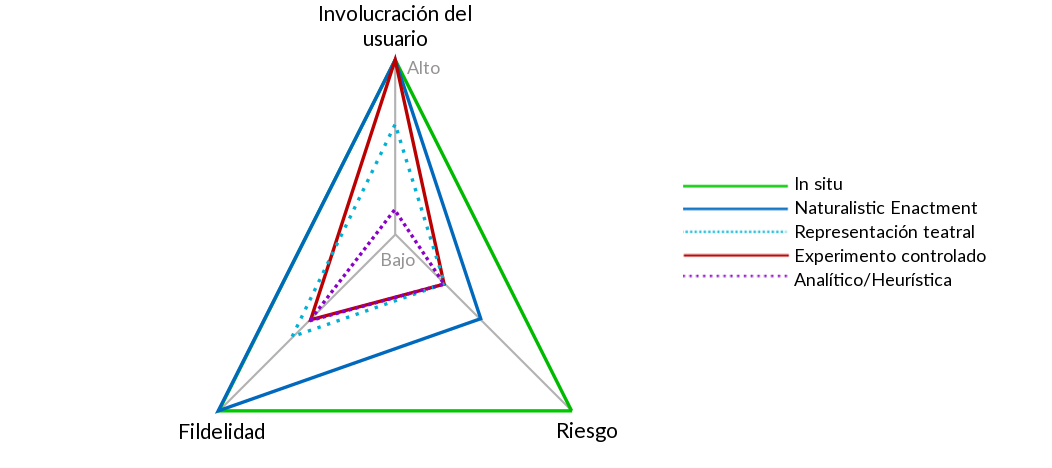
\includegraphics[width=160mm]{./Figures/img_evalmethods}}
        \caption{M\'etodos de evaluaci\'on clasificados de acuerdo a la involucraci\'on del usuario, fidelidad y riesgo}\label{fig:evalmethods}
\end{figure}


Para poder exponer a los sujetos a una situaci\'on de cuidador estresante y realista bajo condiciones controladas, se formul\'o un ejercicio que consisti\'o de una situaci\'on de terapia real con una persona actuando como si tuviera demencia. Un adulto mayor de 75 a\~nos actu\'o como si sufriera de demencia. Se le entren\'o con los comportamientos t\'ipicos de demencia moderada como: murmureo, gritos, vagabundeo, preguntas repetitivas, entre otras. Ella ya estaba familiarazada con estos comportamientos por conocidos que sufrieron de demencia. A los participantes se les dijo que estar\'ian trabajando con una persona que realmente ten\'ia demencia. Tambi\'en, se les ocult\'o la verdadera raz\'on del estudio. En cambio, se les dijo que se evaluaba su rendimiento como cuidadores basados en el entrenamiento inicial que se les di\'o. Para fines pr\'acticos de esta tesis, se referir\'a al adulto mayor como persona con demencia.

Se les pidi\'o firmar un documento de no divulgaci\'on (Ver Ap\'endice~\ref{aped:cartanodiv}) para evitar que los participantes hablaran entre ellos acerca del experimento, de los comportamientos del adulto mayor o cualquier otra t\'ecnica acerca de como manejar el comportamiento del adulto mayor, durante el tiempo en que el experimento durara.

\subsection{Sujetos}\label{secc:subjects}
Los sujetos fueron reclutados a trav\'es de la lista de correo de CICESE (3 personas), por el departamento de ciencias de la computaci\'on (5 personas) y dos personas externas a la instituci\'on. Se les otorg\'o un premio de compensaci\'on de 100.00 MXN en dinero electr\'onico para el cine. Se les pidi\'o a los participantes asisitr a 3 sesiones (una por cada semana), cada sesi\'on requiri\'o al rededor de 90 minutos de su tiempo. Solo pudieron participar personas que no fueran cuidadores formales, y que no fueran cuidadores en el momento. Se incluyeron a personas que tuvieran experiencia como cuidadores informales. Se obtuvo consentimiento firmado de todos los sujetos (Ver Ap\'endice ~\ref{aped:cartainfo})

Todos los sujetos participaron en una sesi\'on de entrenamiento, en donde se les explic\'o las actividades a realizar en las terapias que hicieron con el adulto mayor.
Participaron 10 estudiantes (5 hombres y 5 Mujeres) con un promedio de 24.5 a\~nos de edad ($\sigma=1.059$). La tabla \ref{table:kysymys} muestra los datos demogr\'aficos de los participantes.
\begin{table}
	\footnotesize
	\centering
	\caption{Participantes en el estudio}
	\label{table:kysymys}
	%\rotatebox{90}{
	\begin{tabular}{m{0.2cm}m{2.5cm}m{2.5cm}m{2.5cm}m{2.5cm}}
		\hline\noalign{\smallskip}
		 & \textbf{Sujeto} & \textbf{G\'enero} & \textbf{Edad} & \textbf{Experiencia de cuidador}
		\\ \noalign{\smallskip}
		\hline
		\noalign{\smallskip}
		&S1& Masculino & 24 & No   \\ 
		&S2& Masculino &  25&  No  \\ 
		&S3& Femenino & 24 & No   \\ 
		&S4& Femenino & 26 & No  \\ 
		&S5& Femenino & 24 & No   \\ 
		&S6& Masculino & 26 &  No  \\ 
		&S7& Masculino & 23 &  No \\ 
		&S8& Masculino & 25 &  Si  \\ 
		&S9& Femenino & 26 & No   \\ 
	  	&S10& Femenino & 24 & Si  \\ 
		\hline
	\end{tabular}
	%}
\end{table}
\section{Procedimiento}\label{secc:methods}
El desarrollo del experimento se dividi\'o en diferentes actividades. A continuaci\'on se explican a detalle cada una de ellas.
\subsection{Entrenamiento}\label{secc:training}
Todos los sujetos participaron en una sesi\'on de entrenamiento para familiarizarse con las terapias cognitivas que har\'ian con el adulto mayor. La sesi\'on de entrenamiento dur\'o aproximadamente 90 minutos. Todos los participantes practicaron las terapias y tuvieraon oportunidad de hacer preguntas. No se les di\'o ninguna estrategia de afrontamiento acerca de como lidiar con los coportamientos del adulto mayor. Se les dijo a los participantes que el adulto mayor ten\'ia declive cognitivo ligero y que podr\'ia mostrar algunos problemas de comportamiento como olvidar instrucciones recientes, apat\'ia y renuencia de completar las tareas, entre otras. Se les dijo que las tareas no ten\'ian que ser completadas si el adulto mayor no estaba cooperando, pero que deber\'ian intentar completar la terap\'ia en lo posible.

\subsection{Tareas de terapias}\label{secc:therapytasks}
Antes de iniciar la tarea, equipamos a los participantes con una banda de pecho Zephyr Hxm para monitorizar su ritmo card\'iaco, una pulsera Empatica E3 para obtener GSR y temperatura corporal y una banda cerebral Muse para obtener datos de EEG. Todas las sesiones fueron videograbadas para analizarlas posteriormente.

Durante cinco minutos, ya equipados con los dispositivos, se les pidi\'o a los sujetos relajarase concentrandose en su respiraci\'on con los ojos cerrados para obtener una l\'inea base de datos fisiol\'ogicos. S\'olo una persona necesit\'o mas de 5 minutos.

Se les pidi\'o a los participantes que guiaran al adulto mayor a trav\'es de una sesi\'on de terapia que involucr\'o una de las 7 posibles tareas que fueron explicadas durante la sesi\'on de entrenamiento. La tabla ~\ref{table:therapies} presenta las tareas realizadas por cada participante en las tres sesiones del estudio. La figura ~\ref{fig:imgtherapies} muestra dos terapias de ejemplo. Los rostros de los participantes fueron modificados para mantener su privacidad.

\begin{table}[h!]
	\footnotesize
	\centering
	\caption{Terapias realizadas con el adulto mayor por cada participante.}
	\label{table:therapies}
	%\rotatebox{90}{
	\renewcommand{\arraystretch}{1.5}
	\begin{tabular}{m{0.2cm}m{3.5cm}m{3.5cm}m{3.5cm}m{3.5cm}}
		\hline\noalign{\smallskip}
	&\textbf{Participante}&  \textbf{Terapia 1}& \textbf{Terapia 2}   & \textbf{Terapia 3}  \\ \hline
		\\ \noalign{\smallskip}
		&S1&  Atado de agujetas& Memorama & \pbox{12cm}{Clasificaci\'on\\de im\'agenes}   \\ 
  &S2&  \pbox{12cm}{Clasificaci\'on\\de im\'agenes}& Atado de agujetas & Cruzigrama   \\ 
  &S3&  \pbox{12cm}{Formaci\'on de palabras}& Cruzigrama & Memorama    \\ 
  &S4&  Atado de agujetas&\pbox{12cm}{Clasificaci\'on de\\im\'agenes}& Memorama   \\ 
  &S5&  \pbox{12cm}{Clasificaci\'on\\de im\'agenes}&  Atado de agujetas & Cruzigrama   \\ 
  &S6&  \pbox{12cm}{Separaci\'on de objetos}& Memorama & Atado de agujetas   \\ 
  &S7&  \pbox{12cm}{Separaci\'on de objetos}& Atado de agujetas & Cruzigrama   \\ 
  &S8&  Cruzigrama& Atado de agujetas &\pbox{12cm}{Clasificaci\'on\\de im\'agenes}   \\ 
  &S9&  \pbox{12cm}{Formaci\'on\\de palabras}& \pbox{12cm}{Clasificaci\'on\\de im\'agenes} & Memorama   \\ 
  &S10&  Memorama&\pbox{12cm}{Formaci\'on\\de palabras} & Atado de agujetas   \\ 
		\hline
	\end{tabular}
	%}
\end{table}

\begin{figure}[h!]
        \centering
	\subfigure[]{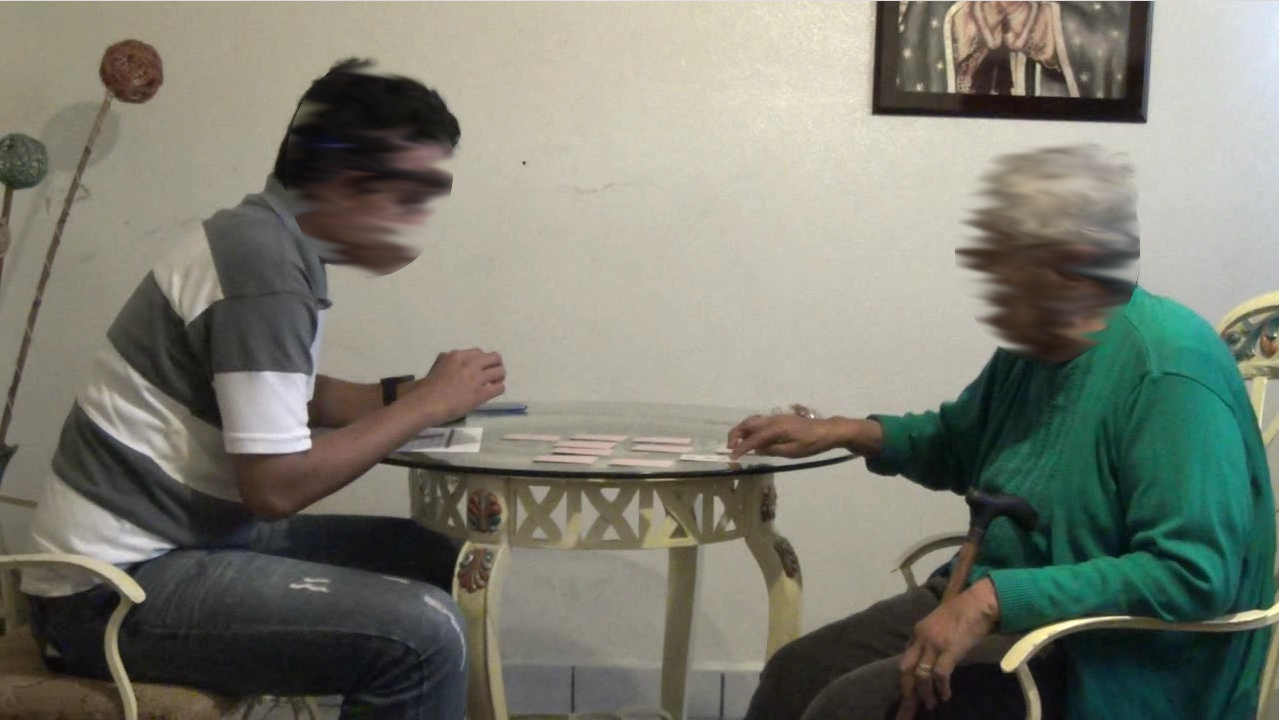
\includegraphics[width=160mm,height=80mm]{./Figures/img_memorama.png}}
	\subfigure[]{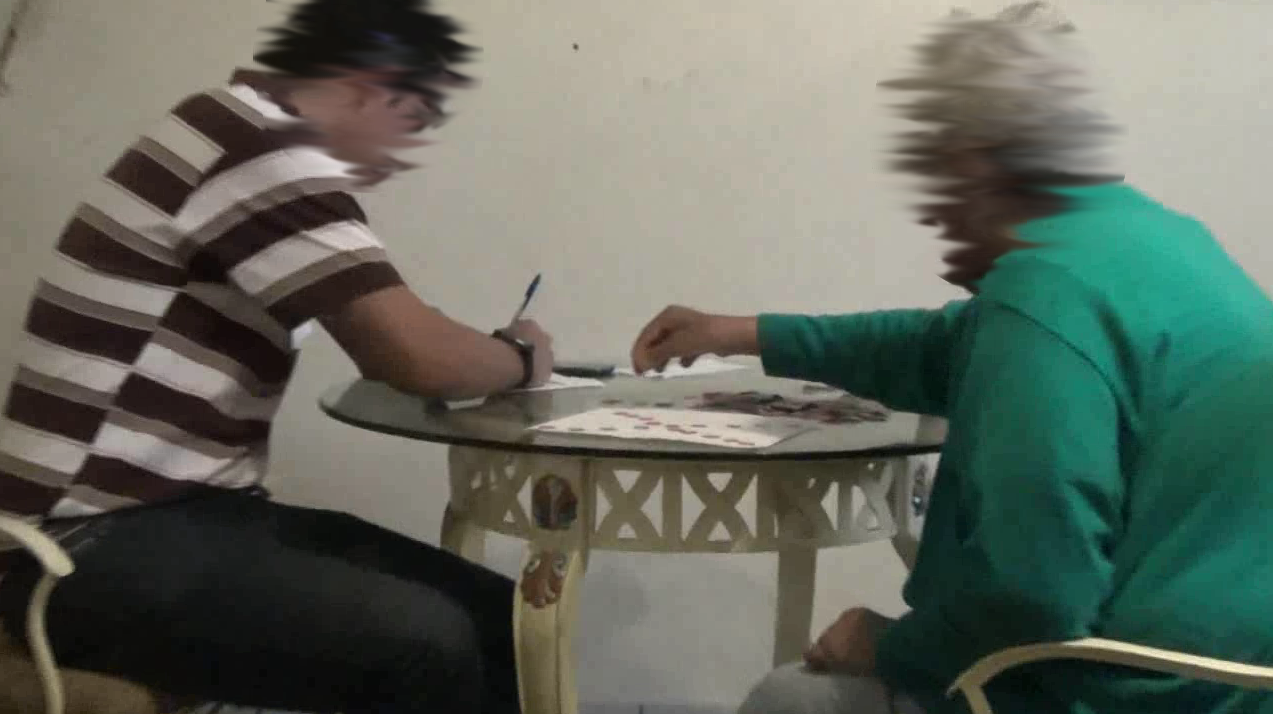
\includegraphics[width=160mm,height=80mm]{./Figures/img_fichas.png}}
	\caption{a) Participante 7 durante una terapia de memorama. b) Participante 7 durante una terapia de separaci\'on de objetos.}\label{fig:imgtherapies}

\end{figure}
%\begin{itemize}
%	\item Atado de agujetas.
%%	\item Separaci\'on de objetos.
%	\item Memorama.
%	\item Clasificaci\'on de im\'agenes.
%	\item Formaci\'on de palabras with syllables.
%	\item Sentences with words.
%	\item Formaci\'on de palabras.
%	\item Cruzigrama.
%\end{itemize}

Toda la intervenci\'on dur\'o 15 d\'ias, cada prueba de los participantes dur\'o alrededor de 30 minutos. Cada d\'ia dos participantes asistieron al sitio.

Cada participante asisiti\'o a tres sesiones. Por cada sesi\'on, una o dos tareas fueron realizadas, con varias iteraciones en cada tarea. Ninguna de las terapias fueron repetidas por los particpantes. Adem\'as, ninguno de los participantes asisti\'o con el mismo compa\~nero mas de una vez.

Se dividi\'o el experimento en tres semanas. Cada sujeto particip\'o una vez cada semana. Se entren\'o al adulto mayor para actuar con diferentes comportamientos diruptivos de distinto nivel de intensidad. En la primer semana, ella actu\'o en niveles de 0 a 2 (Ver tabla ~\ref{table:anxilevels}). En la segunda y tercer semana, actu\'o niveles de 0 a 3. En la \'ultima, se les ense\~n\'o a los participantes a usar estrategias de afrontamiento.
\section{Configuraci\'on}\label{secc:setup}
	Se acondicion\'o un cuarto dentro de una casa real para hacerlo parecer como si fuera la sala de una persona con demencia. La utiler\'ia incluy\'o: Muebles viejos, baja iluminaci\'on, fotograf\'ias viejas, pistas de papel sobre el lavamanos, entre otras. Una mesa de madera fue usada para instalar el equipo: una Macbook, una videoc\'amara, y un tel\'efono inteligente para monitorizar el experimento.
\begin{figure}[h!]
        \centering
        \subfigure[]{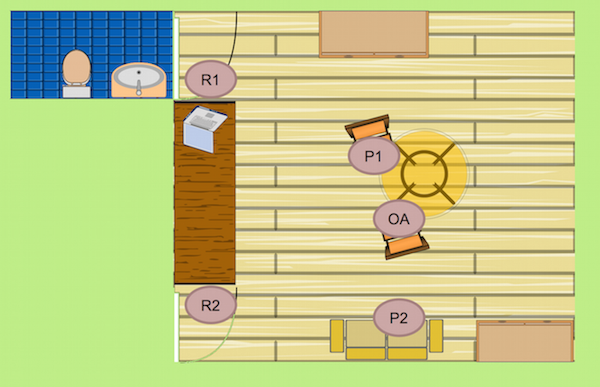
\includegraphics[width=160mm,height=80mm]{./Figures/img_exp_setup}}
	\caption{Escenario del experimento. Las actividades fueron realizadas sobre una mesa, con la persona con demencia (OA) y el participante (P1) sentados frente a frente. El segundo participante (P2) observaba sobre el sof\'a, mientras que dos investigadores (R1,R2) monitoreaban la sesi\'on desde una mesa cercana.} \label{fig:img_exp_setup}
\end{figure}

\begin{figure}[h!]
        \centering
        \subfigure[]{\includegraphics[width=160mm]{./Figures/img_exp_pics}}
	\caption{Fotograf\'ias del escenario real.} \label{fig:img_exp_pics}
\end{figure}
Dos investigadores permanecieron parados al lado de la mesa de madera para operar el equipo y tomar notas (Ver figuras ~\ref{fig:img_exp_setup} y ~\ref{fig:img_exp_pics}). La persona que actuaba como si tuviera demencia y el cuidador permanecieron sentados frente a frente en una mesa circular. Se les pidi\'o a los participantes usar el cuarto de ba\~no para vestir la banda Zephyr debido a que se pone debajo de la ropa, en contacto con la piel. Un segundo participante se sent\'o sobre el sof\'a y le pedimos que observara la sesi\'on. Este participante tambi\'en fue monitorizado por medio de \'unicamente una pulsera Empatica E3.


\subsection{Obtenci\'on de datos}\label{secc:datagathering}
Se desarrollaron dos aplicaciones separadas para el sensor Empatica E3 y el banda Zephyr HxM. Para el primer dispositivo se desarroll\'o la aplicaci\'on ``Care Me Too'' para android (ver figura ~\ref{fig:caremetoo}) la cual se conecta al dispositivo E3 v\'ia Bluetooth Low Energy (BLE), muestra los datos en tiempo real y los guarda en formato .csv. Esta aplicaci\'on tambi\'en puede ayudar a etiquetar eventos con ayuda del usuario, haciendola \'util para estudios naturalistas.


\begin{figure}[h]
        \centering
        \subfigure[]{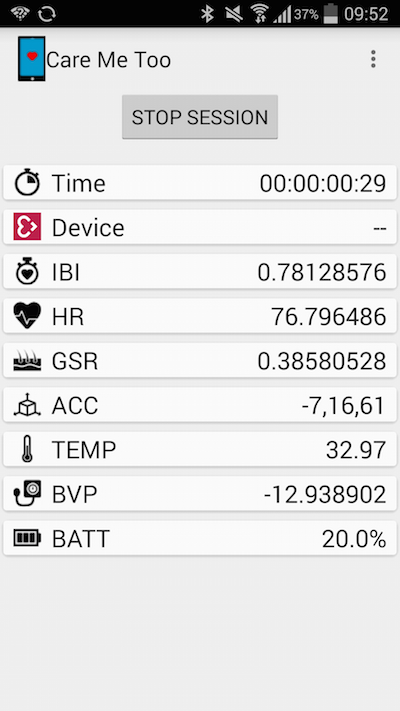
\includegraphics[height=80mm]{./Figures/img_caremetoo}}
        \caption{La aplicaci\'on Care Me Too mostrando se\~nales fisiol\'ogicas siendo grabadas.}\label{fig:caremetoo}
\end{figure}

Para la banda Zephyr HxM se utiliz\'o el programa de l\'inea de comandos ``anxiLogger''\footnote{https://github.com/panzerfausten/anxiLogger} desarrollado por el autor para un estudio anterior \citep{Miranda}. El archivo csv de salida fue agregado a los datos de sesi\'on para sincronizar los tiempos a trav\'es de una librer\'ia llamada ``maxiProcesser''\footnote{https://github.com/panzerfausten/maxiProcesser}
	Para la banda Muse se us\'o la aplicaci\'on de escritorio ``Muse lab'' Los datos obtenidos en formato .muse fueron exportados a .csv para analizarlos posteriormente.

	Se us\'o una laptop Macbook en el sitio para conectar las bandas Muse y Zephyr y un tel\'efono inteligente Samsung Galaxy S4 para colectar datos. Los datos del participante observador fueron obtenidos a trav\'es de una segunda pulsera Empatica E3 en modo de grabaci\'on. Este modo no requiere de una conexi\'on bluetooth.


\section{Obtenci\'on de ground truth}\label{secc:dataanalysis}
Un reto del experimento fue identificar cuando los participantes sent\'ian ansiedad. Para lograrlo, se utilizaron tres diferentes t\'ecnicas: An\'alisis de video, observaci\'on directa y autoreportado. La figura ~\ref{fig:labeling} muestra el proceso unificado de etiquetado. A continuaci\'on se explica el procesado de cada fuente.

\begin{figure}[h]
        \centering
        \subfigure[]{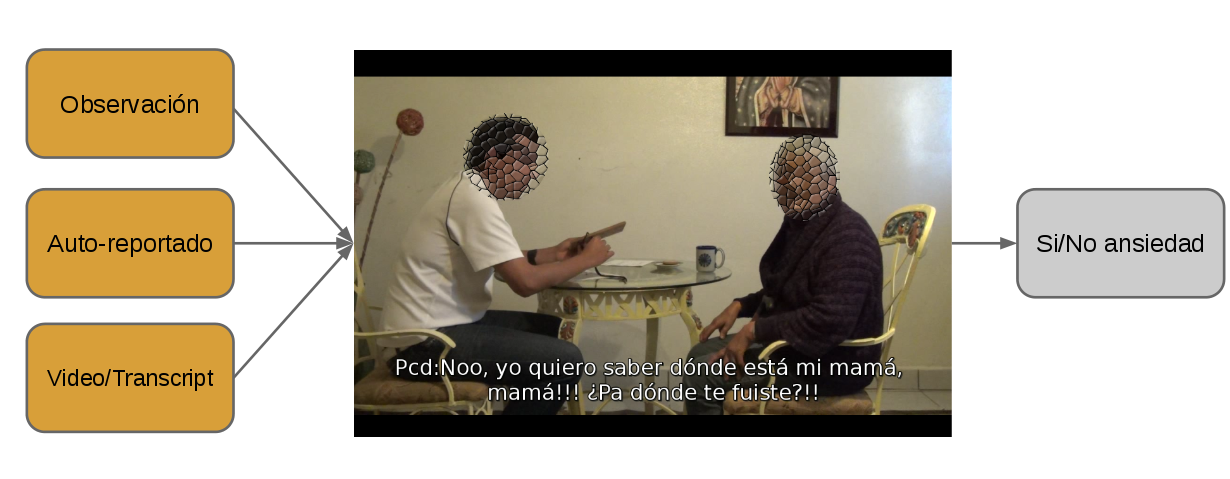
\includegraphics[height=100mm,width=160mm,keepaspectratio]{./Figures/img_labeling}}
	\caption{Proceso de etiquetado a partir de tres diferentes fuentes.}\label{fig:labeling}
\end{figure}
	\subsection{Procesamiento de video}\label{secc:videoprocesing}

	Todos los videos fueron transcritos utilizando el programa F5 transkript para Mac OS X. Con el archivo de transcripci\'on, se generaron subt\'itulos para facilitar el an\'alisis. Luego, se etiquet\'o linea por linea el comportamiento de la persona con demencia. Cada linea fue clasificada en una de los tres posibles niveles que cumplieran con un criterio (ver tabla ~\ref{table:anxilevels}).  La figura ~\ref{fig:f5transcript} muestra una porci\'on de la transcripci\'on de la sesi\'on de un participante
	\begin{table}[h!]
		\footnotesize
		\centering
		\caption{Criterio de etiquetado de comportamiento de la PcD.}
		\label{table:anxilevels}
		%\rotatebox{90}{
		\begin{tabular}{m{2.5cm}m{5.0cm}m{5.0cm}m{2.5cm}}
			\hline\noalign{\smallskip}

		    \textbf{Nivel} & \textbf{Criterio}                                                                                    & \textbf{Ejemplo de evento}                                                                      \\ \hline
			\\ \noalign{\smallskip}

			    0     & \pbox{12cm}{La PcD actua de forma pasiva,\\La PcD accede a participar,  \\El participante y la PcD \\est\'an haciendo la tarea} &                   \pbox{12cm}{La PcD est\'a realizando la\\ tarea como se le pidi\'o.}                       \\ 
	      1     & \pbox{12cm}{Comportamientos renuentes.,\\Reacio a participar,\\Quejandose acerca de la tarea.}                & \pbox{12cm}{ ``No me gusta este juego.'' \\ ``Esto es muy dif\'icil.'' \\``Hazlo tu.'' }             \\ 
	      2     & \pbox{12cm}{Murmureo,\\Hablando cosas sin sentido,  \\Comportamientos impredecibles}                                      & \pbox{5cm}{``?`Donde est\'a mi mam\'a?''\\``Qui\'en eres?''}                                          \\ 
	      3     & \pbox{12cm}{Gritos.\\Amenazas al particpante,\\Paranoia,  \\Urgencia de irse.}                          & \pbox{12cm}{``MAM\'A, DONDE EST\'AS!!??''\\``YA QUIERO IRME!''  \\``QUIEN ERES? D\'EJAME IR!'' } \\ 
			\hline
		\end{tabular}
		%}
	\end{table}
\begin{figure}[h!]
        \centering
        \subfigure[]{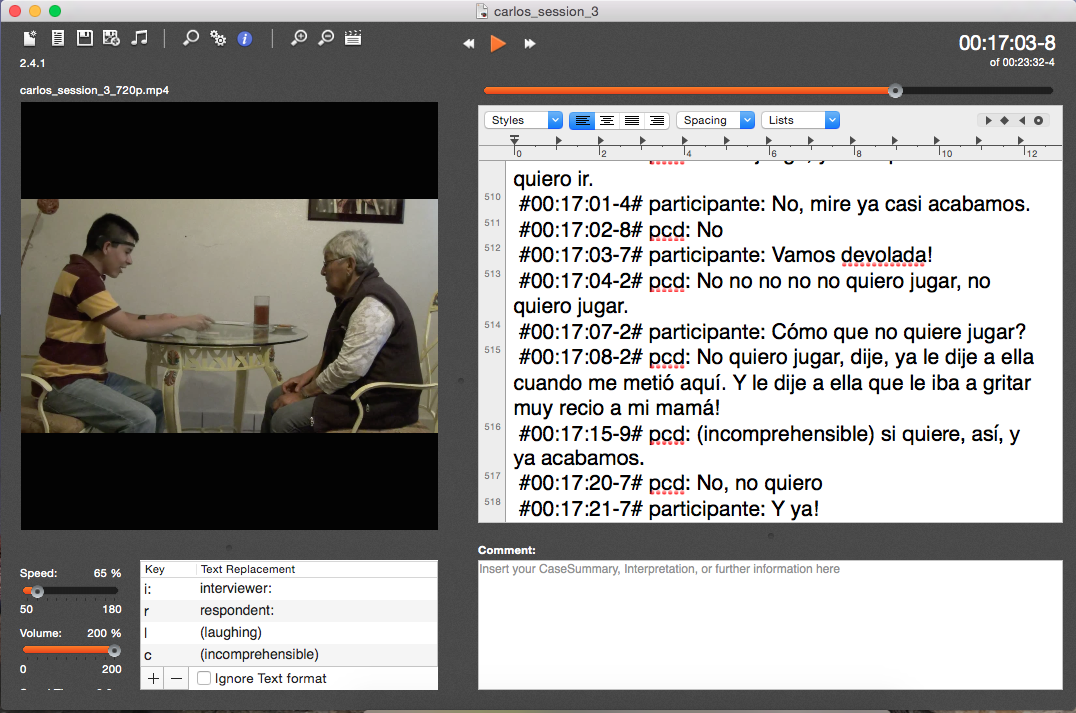
\includegraphics[height=10cm,keepaspectratio]{./Figures/img_transcript.png}}
        \caption{Transcripci\'on correspondiente a una sesi\'on completa de un participante}\label{fig:f5transcript}
\end{figure}

%La figura ~\ref{fig:imgsegment} ejemplifica un segmento extra\'ido. En el siguiente cap\'itulo se explica como se clasificaron los datos y los resultados de la detecci\'on.

%\begin{figure}[h]
%        \centering
%        \subfigure[]{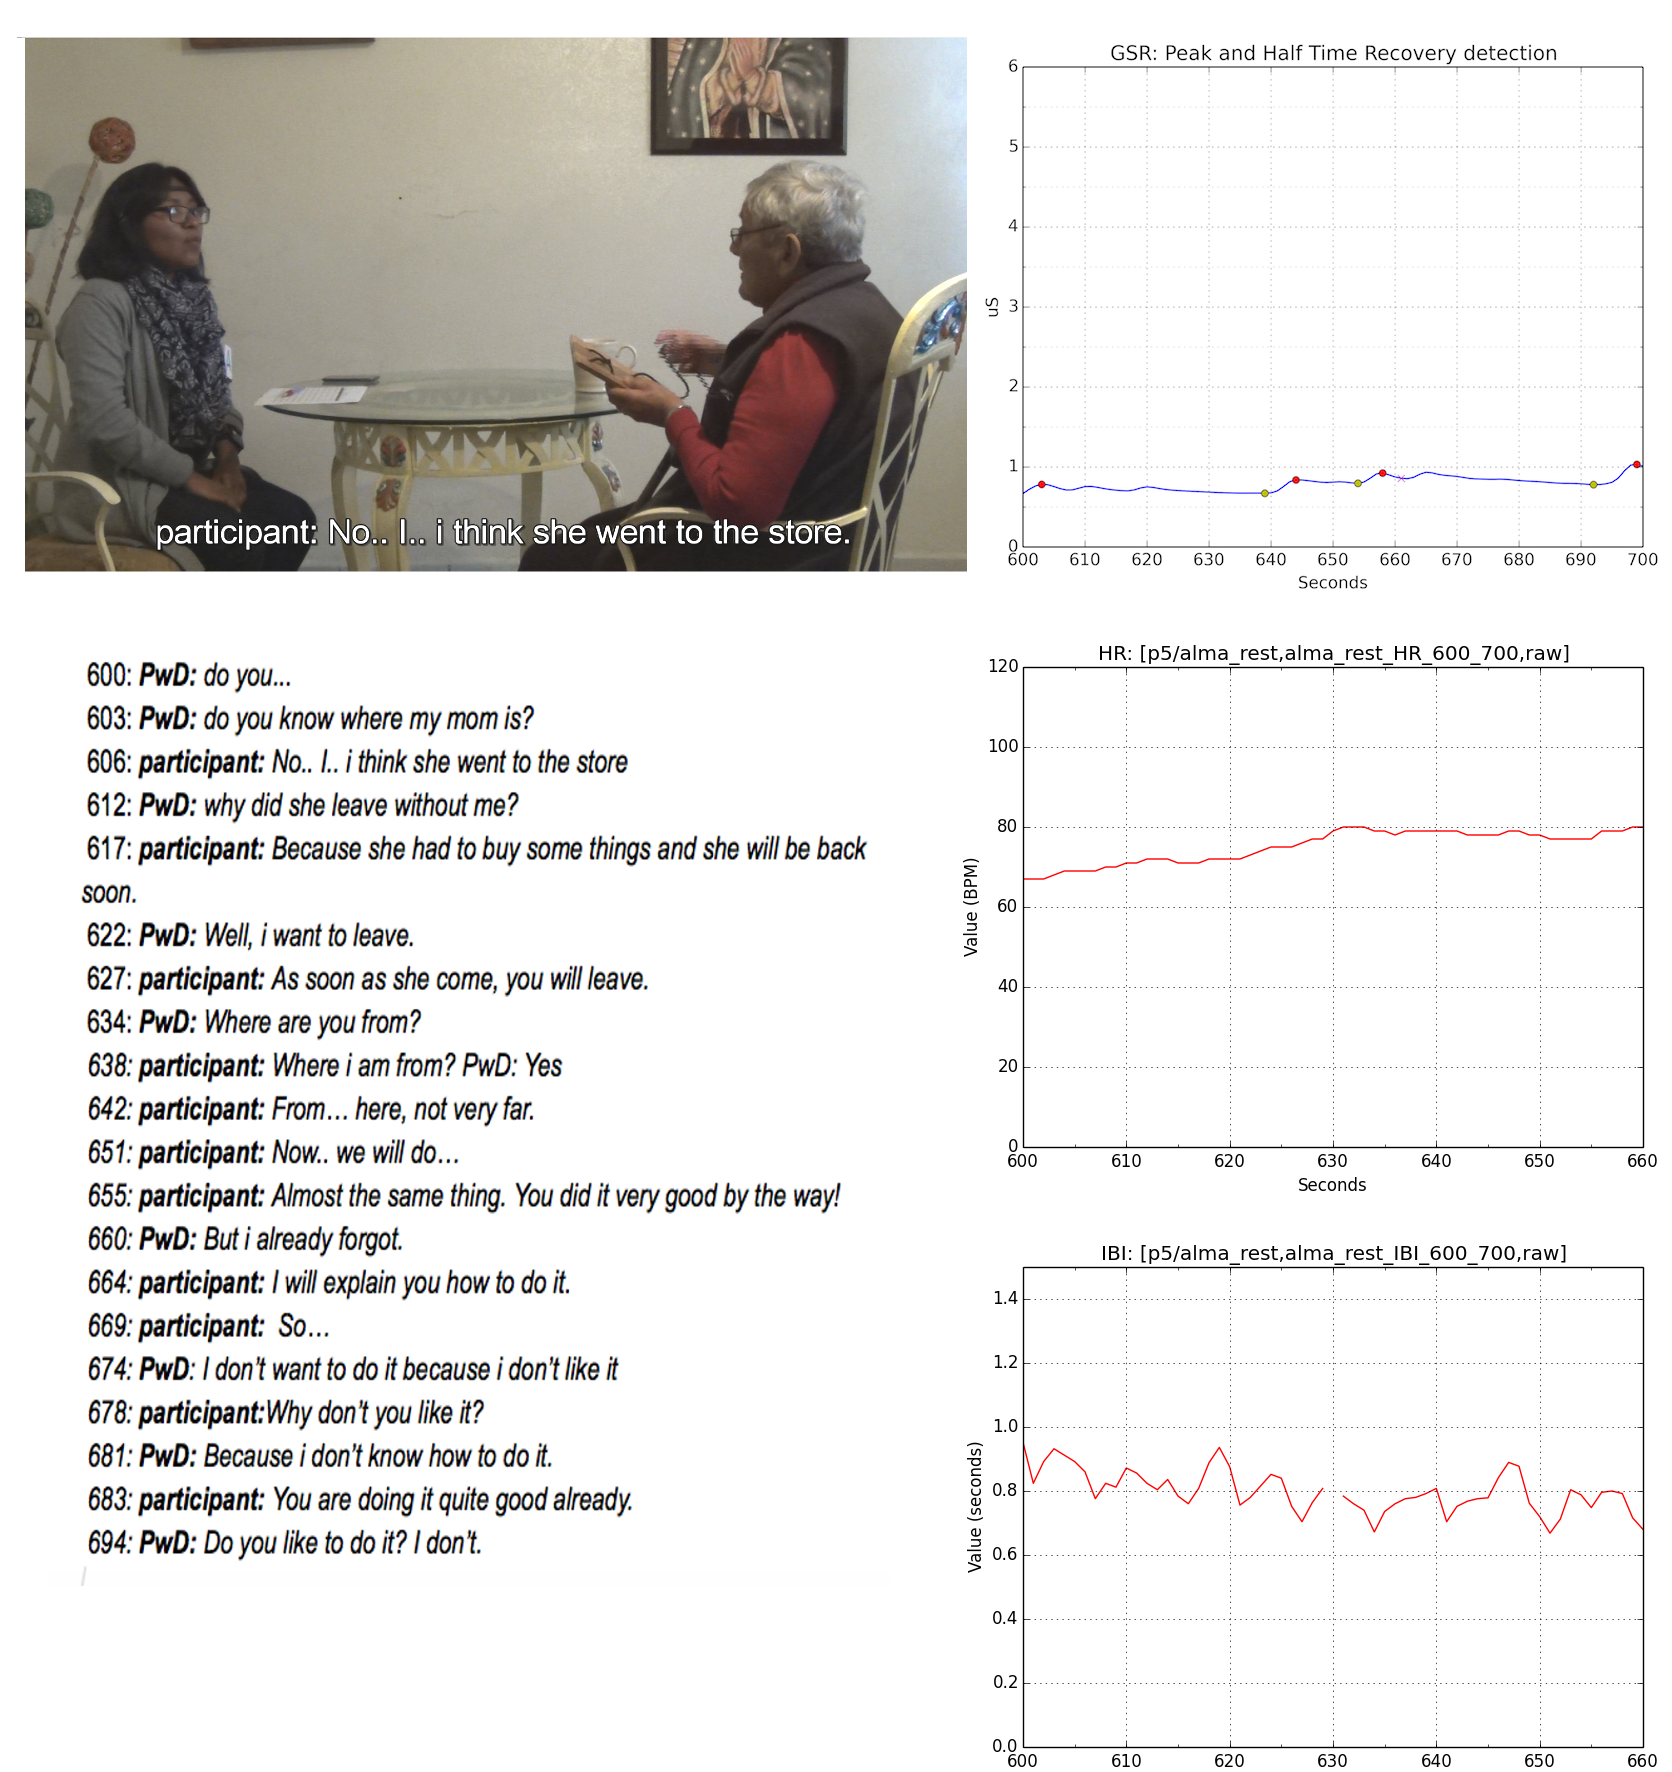
\includegraphics[height=18cm,keepaspectratio]{./Figures/img_segment.png}}
%        \caption{Transcripci\'on y se\~nales GSR, HR, e IBI correspondientes a una situaci\'on estresante}\label{fig:imgsegment}
%\end{figure}

	\subsection{Observaci\'on}
	Dos investigadores realizaron observaci\'on en el sitio, tomando nota del tiempo, nivel del comportamiento de la persona con demencia, y una descripci\'on del evento. Esta descripci\'on fue escrita en base a lo que el participante y/o la persona con demencia dijo o hizo en el momento. El nivel de comportamiento fue codificado en base a la tabla ~\ref{table:anxilevels}. Un evento etiquetado como ``0'' corresponde a cuando la persona con demencia se encuentra realizando la tarea como se le pidi\'o. En esta situaci\'on el cuidador puede estar totalmente relajado o bien ligeramente estresado. En un evento con la etiqueta ``1'' la PcD se encuentra en un estado renuente diciendo cosas como ``No me gusta esta tarea'' o ``Hazlo tu, yo no quiero''. La PcD podr\'ia estar realizando la tarea con bajo rendimiento o podr\'ia no prestar atenci\'on del todo. En un nivel ``2'', la PcD realiza situaciones no esperadas como preguntar al participante por su madre o cualquier otra pregunta que lo ponga inc\'omodo. La atenci\'on hacia la tarea puede ser muy baja. En el nivel ``3'', la PcD realiza acciones como tratar de golpear al participante, levantarse de la silla y querer salir de la habitaci\'on o gritar. La atenci\'on a la tarea suele ser nula. La figura~\ref{fig:imgobservation} ejemplifica la observaci\'on correspondiente a una sesi\'on.

\begin{figure}[h]
        \centering
        \subfigure[]{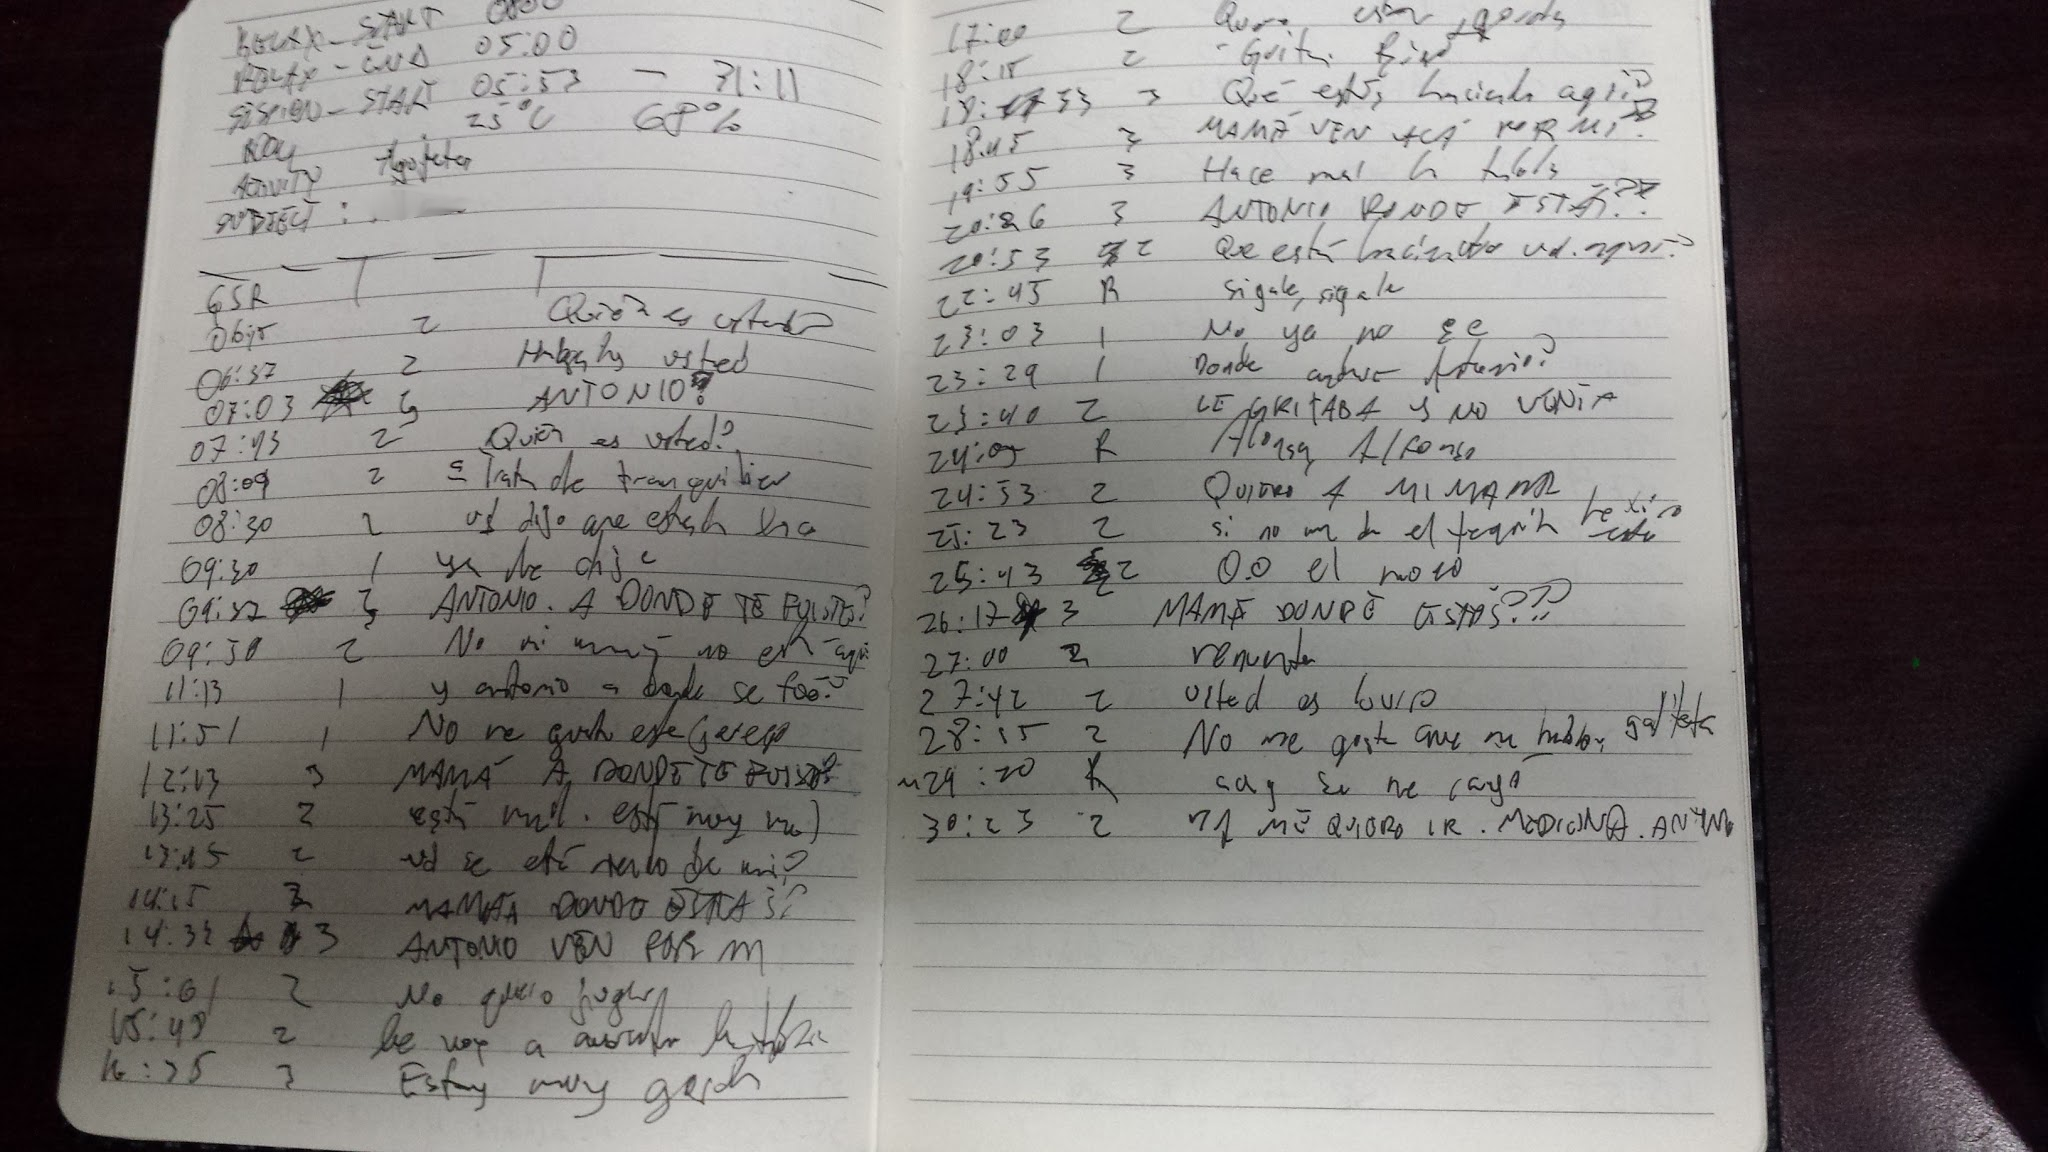
\includegraphics[height=200mm,width=160mm,keepaspectratio]{./Figures/img_observation.png}}
        \caption{Libreta de observaci\'on. Se anot\'o el tiempo con respecto al inicio de la sesi\'on, el nivel de evento de la PcD percibido y una porci\'on del dialogo como referencia. Otros datos como la temperatura y humedad relativa del cuarto fueron anotados.}\label{fig:imgobservation}
\end{figure}
	\subsection{Autoreportado}
	Se les entreg\'o a los participantes un formulario en papel para indicar su nivel de ansiedad mientras desarrollaban la tarea. Se les explic\'o a los participantes durante la sesi\'on de entrenamiento como utilizar el formulario de auto reportado. Sin embargo, algunos de ellos encontraron dif\'icil de contestarlo adecuadamente, principalmente porque estaban muy ocupados con la terapia. La figura ~\ref{fig:imggtlabel} ejemplifica el auto reportado de un participante que contest\'o correctamente el formulario.
	\begin{figure}[h!]
		\centering
		\subfigure[]{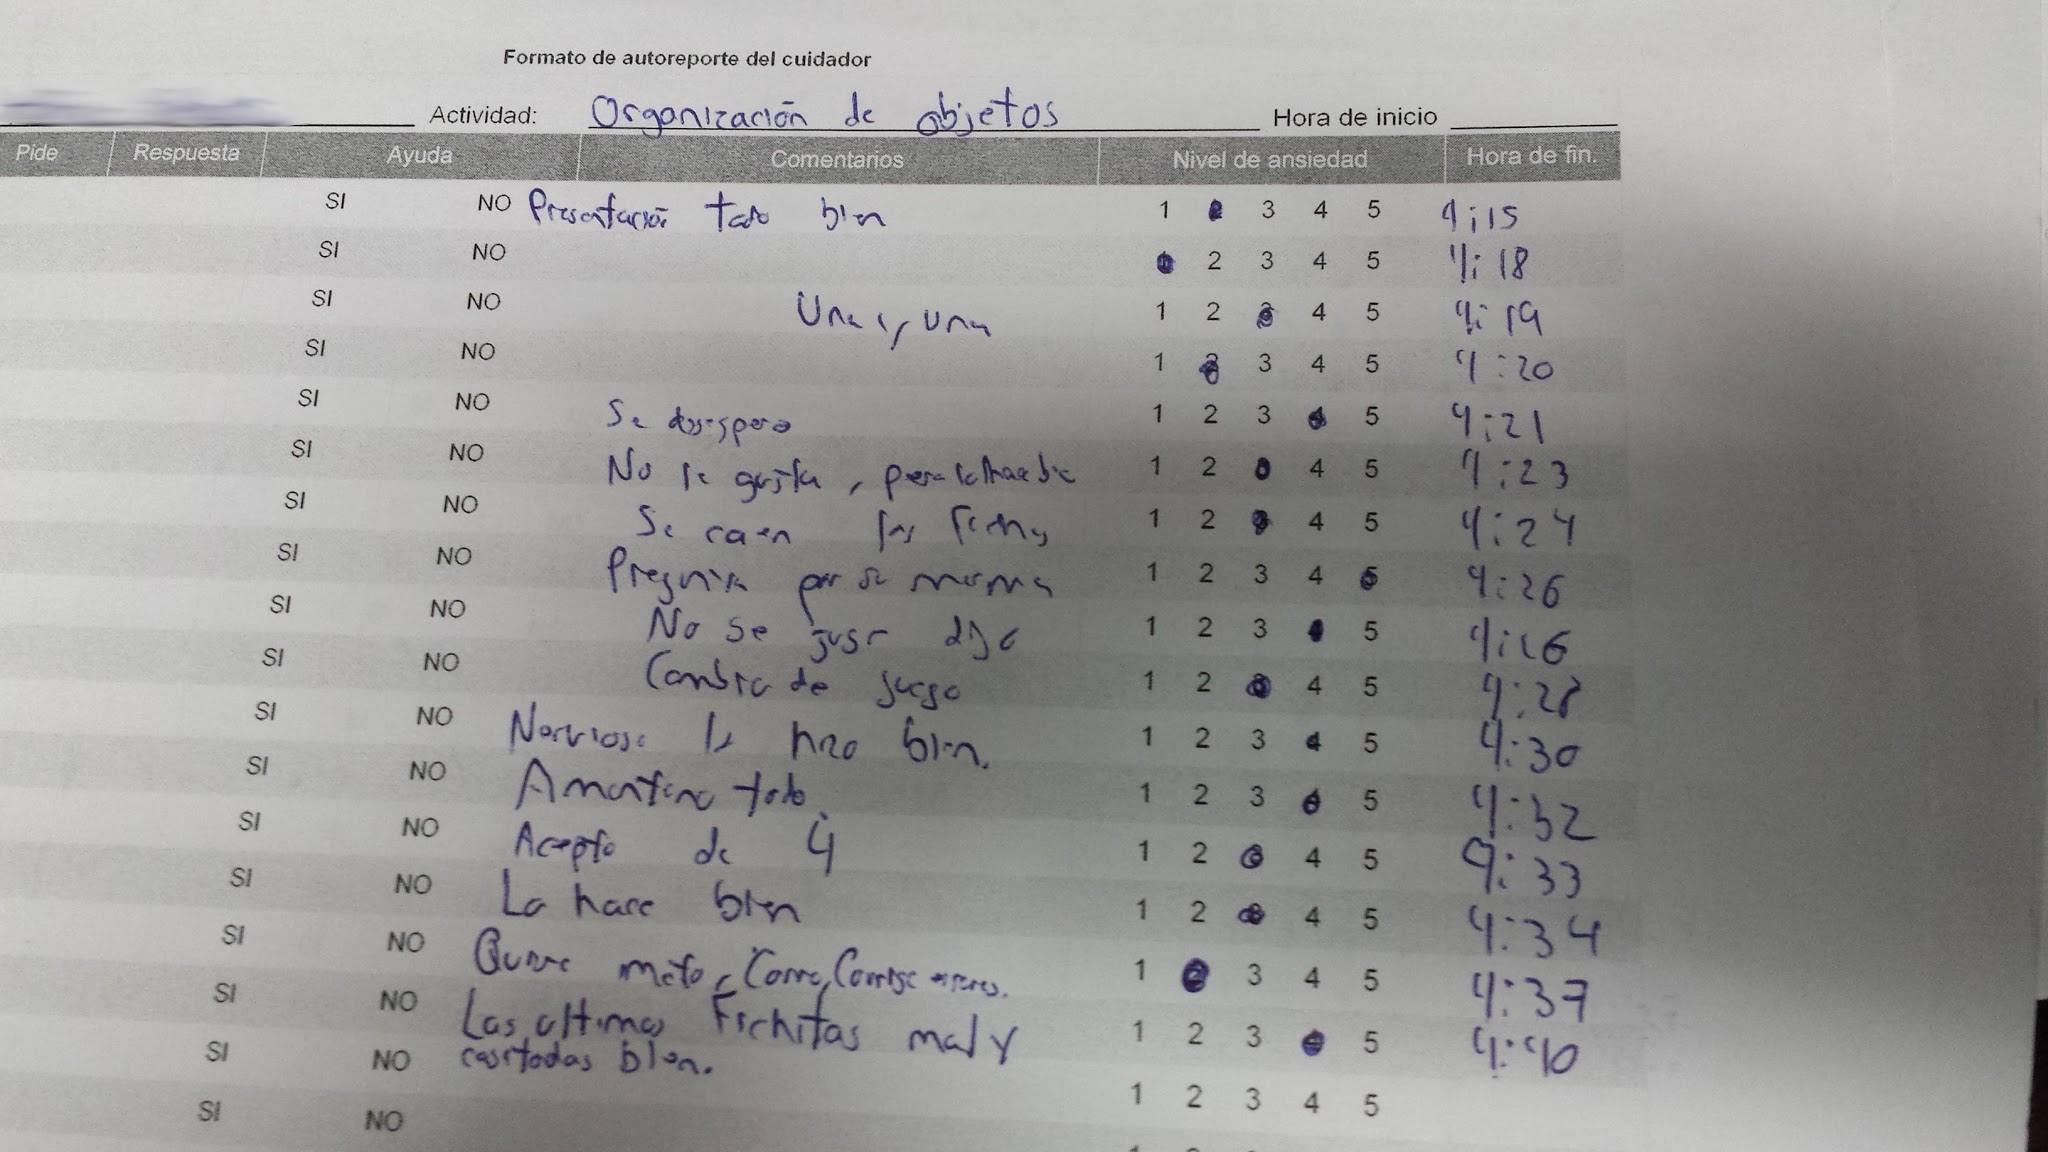
\includegraphics[height=200mm,width=160mm,keepaspectratio]{./Figures/img_sr.png}}
		\caption{Formato de auto reportado de una sesi\'on completa de un participante}\label{fig:imggtlabel}
	\end{figure}

	\subsection{Unificaci\'on de ``ground truth''}
	Por \'ultimo, se gener\'o un formato con los datos de transcripci\'on, nivel del evento de la persona con demencia y auto reportado. Al mismo tiempo, se observ\'o el video para obtener rasgos de ansiedad como cambios en la tonalidad de voz, desv\'io de mirada, o movimientos del participante. Con esta informaci\'on, se etiquet\'o cada 30 segundos si exist\'ia ansiedad o no. Se anot\'o con el n\'umero ``1'' cuando claramente el participante experimentaba ansiedad y con un ``0'' si claramente no. Si el segmento era muy ambiguo (p. ej. El participante se ve ansioso en el video pero el nivel del auto reportado y el evento de la PcD eran bajos) se etiquet\'o con el n\'umero ``-1''. La figura ~\ref{fig:imggtlabel} ejemplifica un segmento codificado.
	\begin{figure}[h!]
		\centering
		\subfigure[]{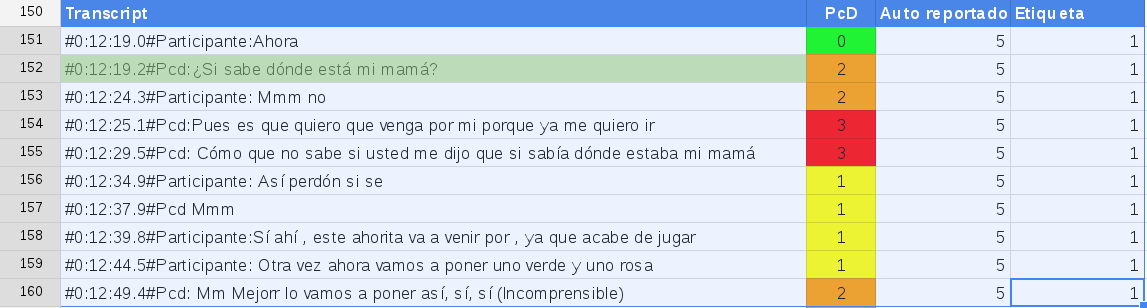
\includegraphics[height=200mm,width=160mm,keepaspectratio]{./Figures/img_gtlabel.png}}
		\caption{Segmento codificado como ansiedad. El nivel de auto reportado es alto y existen valores altos en el comportamiento de la PcD. }\label{fig:imggtlabel}
	\end{figure}
\section{Preprocesamiento de GSR}\label{secc:gsrpreprocessing}
Se desarroll\'o una librer\'ia en python para procesar todos los datos fisiol\'ogicos, incluyendo funciones para exportar, extraer caracter\'isticas, sincronizaci\'on de tiempos, y graficado de datos de ansiedad de todos los dispositivos. La librer\'ia tambi\'en puede graficar atributos de la se\~nal GSR (picos, tiempos de recuperaci\'on medios, amplitudes, etc.) y guardar los datos en formato .csv y .json.

Se inici\'o remuestreando los datos de GSR de 4.0 Hz a 1.0 Hz calculando el valor promedio de todos los datos que cayeran en una ventana deslizante de 1 segundo. Esto se hizo debido a que se esperaba que los periodos de ansiedad duraran segundos. Luego, se aplic\'o un filtro gausiano para suavizar la se\~nal y el ruido. Finalmente, se us\'o un m\'etodo de la librer\'ia scipy de python para detectar picos y se filtraron todos los picos con amplitud mas grande que un umbral ($t \geqslant 0.04$ para datos no normalizados y $t \geqslant 0.01$ para datos normalizados). Tambi\'en se calcul\'o el ``Tiempo de media recuperaci\'on'' de la se\~nal. Esto es, el punto donde la se\~nal decae al valor exacto de la mitad del pico.
\section{Preprocesamiento de HR e IBI}\label{secc:hribipreprocessing}
No fue necesario remuestrear los datos de HR e IBI debido a la naturaleza de la se\~nal. El sensor solo reporta datos cuando ocurre un latido del coraz\'on. Sin embargo, se agrup\'o en ventanas de segundos para compararlo con el resto de las se\~nales. El ruido de los datos fu\'e muy bajo y no requiri\'o pre-procesamiento adicional.
\section{Extracci\'on de caracter\'isticas}
Una vez segmentadas y etiquetadas las sesiones, se tomaron varias caracter\'isticas por cada tipo de se\~nal. Estas caracter\'isticas generalizan al evento completo. La tabla ~\ref{tab:features} describe dichas caracter\'isticas.

	\begin{table}[t]
		\footnotesize
		\centering
        	\caption{Caracter\'isticas usadas como entrada para el clasificador de SVM}
 	       \label{tab:features}

		%\rotatebox{90}{
		\begin{tabular}{m{2.5cm}m{5.0cm}m{5.0cm}m{2.5cm}}
			\hline\noalign{\smallskip}

                \textbf{Se\~nal} & \textbf{Caracter\'istica} & \textbf{Descripci\'on} & \textbf{Unidad} \\
		\hline
			\\ \noalign{\smallskip}
                GSR   & \pbox{12cm}{\textit{Amplitud de los picos}}                & \pbox{12cm}{Distancias promedio \\desde el punto de crecimiento\\ hacia el pico}             & \pbox{12cm}{$\mu S$}        \\
                GSR   & \pbox{12cm}{\textit{Amplitud m\'axima de los picos}}                & \pbox{12cm}{Amplitud mas grande \\ de los picos}             & \pbox{12cm}{$\mu S$}        \\
                GSR   & \pbox{12cm}{\textit{Amplitud m\'inima de los picos}}                & \pbox{12cm}{Amplitud mas chica \\ de los picos}             & \pbox{12cm}{$\mu S$}        \\
                GSR   & \pbox{12cm}{\textit{Varianza de los picos}}                & \pbox{12cm}{Varianza total de todos\\ los picos}             & \pbox{12cm}{$\mu S$}        \\
			GSR   & \pbox{12cm}{\textit{Tiempo promedio de} \\\textit{media recuperaci\'on de los picos}}                & \pbox{12cm}{Varianza total de todos\\ los picos}             & \pbox{12cm}{$\mu S$}        \\
                IBI   &\textit{M\'inimo}                & Valor m\'inimo del segmento            &Segundos       \\
                IBI   &\textit{M\'aximo}                & Valor m\'aximo del segmento            &Segundos       \\
                IBI   &\textit{Promedio}                & Valor promedio del segmento            &Segundos       \\
                IBI   &\textit{Desviaci\'on estandar}                &  \pbox{12cm}{Desviaci\'on estandar de todos\\ los datos del segmento}            &Segundos        \\


        \end{tabular}
\end{table}
%TODO:UPDATE THIS 
%Para este trabajo, se tuvo un total de 51 segmentos del nivel 0, 177 del nivel 1, 145 del nivel 2 y 106 del nivel 3. Los datos corresponden a 5 del total de 10 de participantes. Utilizando 15 sesiones. No se procesaron todas las sesiones en su totalidad, debido al extenso tiempo necesario para transcribir los videos. Todos los segmentos fueron luego codificados en forma de vectores descriptores. Estos vectores fueron guardados en formato .csv, con la primera columna correspondiente a la etiqueta de nivel de ansiedad.
%\section{Sincronizaci\'on de datos}
%	Agregar 
\section{Conclusi\'on}
El dise\~no de este experimento permite recabar datos de cuidadores de personas con demencia en situaciones naturalistas. El riesgo es reducido al utilizar situaciones simuladas que los participantes piensan que son reales. Esto abre la posibilidad de analizar por medio de tecnolog\'ia los efectos de ansiedad en los cuidadores.
En la siguiente secci\'on se utiliza una t\'ecnica de aprendizaje de m\'aquina para clasificar los eventos de ansiedad. Se explican las diferentes pruebas realizadas, y los resultados generales de este experimento.
\newpage
%%=====================================================

